\documentclass[12pt,a4paper]{report}
\usepackage[none]{hyphenat}
\usepackage{setspace}
\usepackage[left=3.7cm,right=2.5cm,top=2.5cm,bottom=2.5cm]{geometry}
\usepackage{amsmath}
\usepackage{url}
\usepackage{graphicx}
\usepackage{float}
\usepackage[toc,page]{appendix}
\usepackage{multirow}
\usepackage{titling}
\usepackage{acro}
\usepackage{subcaption}
\usepackage{array}
\usepackage{dirtytalk}
\usepackage{listings}

% Default fixed font does not support bold face
\DeclareFixedFont{\ttb}{T1}{txtt}{bx}{n}{11} % for bold
\DeclareFixedFont{\ttm}{T1}{txtt}{m}{n}{11}  % for normal

% Custom colors
\usepackage{color}
\definecolor{deepblue}{rgb}{0,0,0.5}
\definecolor{deepred}{rgb}{0.6,0,0}
\definecolor{deepgreen}{rgb}{0,0.5,0}
\definecolor{deepgrey}{rgb}{0.329, 0.431, 0.478}

% Python style for highlighting
\newcommand\pythonstyle{\lstset{
    language=Python,
    basicstyle=\tiny\ttm,
    otherkeywords={self},            
    keywordstyle=\ttb\color{deepblue},
    emph={MyClass,__init__},          % Custom highlighting
    emphstyle=\ttb\color{deepred},    % Custom highlighting style
    stringstyle=\ttm\color{deepgreen},
    commentstyle=\ttm\color{deepgrey},
    frame=tb,                        
    showstringspaces=false,          
    breaklines=true,
    postbreak=\mbox{\textcolor{red}{$\hookrightarrow$}\space},
}}


% Python environment
\lstnewenvironment{python}[1][]
{
    \pythonstyle
    \lstset{#1}
}{}

% Python for external files
\newcommand\pythonexternal[2][]{{
\pythonstyle
\lstinputlisting[#1]{#2}}}

% Python for inline
\newcommand\pythoninline[1]{{\pythonstyle\lstinline!#1!}}

\author{M.A.P.P. Marasinghe}

\linespread{2}
\graphicspath{ {images/} }

\DeclareAcronym{stft}{
  short = STFT,
  long  = Short Time Fourier Transformation
}
\DeclareAcronym{sift}{
  short = SIFT,
  long  = Scale Invariant Feature Transform
}
\DeclareAcronym{dog}{
  short = DoG,
  long  = Difference of Gaussians
}
\DeclareAcronym{blob}{
  short = BLOB,
  long  = Binary Large Object
}
\DeclareAcronym{osca}{
  short = OSCA,
  long  = Outstanding Song Creators Association
}

\DeclareAcronym{pca}{
  short = PCA,
  long  = Principle Component Analysis
}

\DeclareAcronym{mir}{
  short = MIR,
  long  = Music Information Retrival
}

\DeclareAcronym{pcp}{
  short = PCP,
  long  = Pitch Class Profiles
}

\DeclareAcronym{oti}{
  short = OTI,
  long  = Optimal Transposition Index
}

\DeclareAcronym{dp}{
  short = DP,
  long  = Dynamic Programming
}

\DeclareAcronym{dtw}{
  short = DTW,
  long  = Dynamic Time Warping
}

\DeclareAcronym{svd}{
  short = SVD,
  long  = Singular Value Decomposition
}

\DeclareAcronym{tp}{
  short = TP,
  long  = True Positive
}

\DeclareAcronym{fp}{
  short = FP,
  long  = False Positive
}

\DeclareAcronym{tn}{
  short = TN,
  long  = True Negative
}

\DeclareAcronym{fn}{
  short = FN,
  long  = False Negative
}






\begin{document}

\begin{titlepage}
    \begin{center}

        % \includegraphics[width=3cm]{uoc.png}\\
        % \vspace{24pt}
        % \textbf{\Huge{Protecting Copyright Ownership via Identification of Remastered Music in Radio Broadcasts}}


        % \vspace{36pt}
        % \textbf{{\Large{M. A. P. P. Marasinghe}}}\\
        % \textbf{{\Large{Index No : 15000877}}}\\

        % \vspace{36pt}
        % \textbf{{\Large{Supervisor : Dr. K.L. Jayaratne}}}\\
        % \textbf{{\Large{Co-supervisor : Dr. M.I.E. Wickramasinghe}}}\\

        % \vspace{60pt}
        % \textbf{{\Large{February 2020}}}\\
        
        % \vspace{12pt}
        % \singlespacing
        % \large {Submitted in partial fulfillment of the requirements of the}\\
        % \large {B.Sc in Computer Science Final Year Project (SCS4124)}
        
        % \vspace{24pt}
        % \includegraphics[width=3.5cm]{Ucsc.jpg}\\

Protecting Copyright Ownership via Identification of Remastered Music in Radio Broadcasts

\vspace{12pt}

By

\vspace{12pt}

M. A. P. P. Marasinghe \\
2015/CS/087

\vspace{140pt}


This dissertation is submitted to the University of Colombo School of Computing \\
In partial fulfillment of the requirements for the \\
Degree of Bachelor of Science Honours in Computer Science


\vspace{140pt}


University of Colombo School of Computing \\
35, Reid Avenue, Colombo 07, \\
Sri Lanka \\
July 2020


    \end{center}
\end{titlepage}
\clearpage

\linespread{2}
%\begin{titlepage}
    \begin{center}
        \textbf{\Huge{Protecting Copyright Ownership via Identification of Remastered Music in Radio Broadcasts}}
        \vfill
        \huge{M.A.P.P. Marasinghe}
    \end{center}
\end{titlepage}

\pagenumbering{roman}
\onehalfspacing
\sloppy

\chapter*{Declaration}
\addcontentsline{toc}{chapter}{Declaration}

I, M. A. P. P. Marasinghe (2015/CS/087) hereby certify that this dissertation entitled “Protecting Copyright Ownership via Identification of Remastered Music in Radio Broadcasts” is entirely my own work and it has never been submitted nor is currently been submitted for any other degree.


\vspace{1.75cm}
\noindent
\makebox[130pt]{\dotfill}\hspace{120pt}\makebox[150pt]{\dotfill} \\
\mbox{}\hspace{50pt}Date \hspace{190pt} M. A. P. P. Marasinghe  


\vspace{1cm}
\noindent
I, Dr. K. L. Jayaratne, certify that I supervised this dissertation entitled “Protecting Copyright Ownership via Identification of Remastered Music in Radio Broadcasts” conducted by M. A. P. P. Marasinghe in partial fulfillment of the requirements for the degree of Bachelor of Science Honours in Computer Science. 


\vspace{1.75cm}
\noindent
\makebox[130pt]{\dotfill}\hspace{120pt}\makebox[150pt]{\dotfill} \\
\mbox{}\hspace{50pt}Date \hspace{200pt} Dr. K.L. Jayaratne 

\vspace{1cm}
\noindent
I, Dr. M.I.E. Wickramasinghe, certify that I co-supervised this dissertation entitled “Protecting Copyright Ownership via Identification of Remastered Music in Radio Broadcasts” conducted by M. A. P. P. Marasinghe in partial fulfillment of the requirements for the degree of Bachelor of Science Honours in Computer Science. 

\vspace{1.75cm}
\noindent
\makebox[130pt]{\dotfill}\hspace{120pt}\makebox[150pt]{\dotfill} \\
\mbox{}\hspace{50pt}Date \hspace{170pt} Dr. M.I.E. Wickramasinghe 
\clearpage

\chapter*{Abstract}
\addcontentsline{toc}{chapter}{Abstract}

Music identification in radio broadcasts have different use cases like playlist generation
and protecting copyright ownership of artistes. In real world environments, music is often
remastered by radio channels to fit in to limited air times. Mostly those remastering
includes time stretching, pitch shifting and etc. Therefore robustness of the music identification
method plays a crucial role. 
\vspace{12pt}

In this dissertation, we propose to use \ac{sift} on \ac{stft} spectrogram to extract audio
descriptors. Experiments show that \ac{sift} descriptors exhibit robustness against audio 
distortions such as time stretching and pitch shifting. Finally a ratio based threshold is
used to differentiate identified and non-identified states.  

\chapter*{Preface}
\addcontentsline{toc}{chapter}{Preface}

The new method of remastered music identification method introduced
in this research is a method refined by me in conjunction with my supervisor
and co-supervisor. The song registration module, database structure and 
audio matching module are  my own work. The results of the Section \ref{section:results}
rely upon experiments conducted by me. 

\chapter*{Acknowledgement}
\addcontentsline{toc}{chapter}{Acknowledgement}

I would like to express my very great appreciation to Dr. K.L. Jayaratne, my research supervisor for his valuable guidance, 
support and encouragement throughout this research work.
\vspace{12pt}

I would also like to give special thanks to my co-supervisor Dr. M.I.E. Wickramasinghe for his valuable and constructive 
suggestions during the planning and development of this research work and for his patient guidance and assistance in keeping 
my progress on schedule. Also his willingness to give his time so generously has been very much appreciated.
\vspace{12pt}

My special thanks are extended to the staff of Outstanding Song Creators Association (OSCA) for their assistance with the 
collection of my data.
\vspace{12pt}

I wish to acknowledge the help provided by my examiners Prof. G.K.A. Dias and Dr. M.G.N.A.S. Fernando for their valuable 
feedback in every evaluation to help me improve my work.
\vspace{12pt}

Finally, I wish to thank my beloved parents for their support, encouragement and being there for me in all my hardships. 



\renewcommand\contentsname{Table of Contents\\}
\onehalfspacing
\linespread{1}
\tableofcontents
\clearpage

\listoffigures
\addcontentsline{toc}{chapter}{List of Figures}

\listoftables
\addcontentsline{toc}{chapter}{List of Tables}

\printacronyms[heading=chapter*, name=List of Acronyms]
\addcontentsline{toc}{chapter}{List of Acronyms}
\clearpage

\pagenumbering{arabic}

\chapter{Introduction}
\section{Background to the Research}
\vspace{12pt}

According to the intellectual property act of Sri Lanka\cite{CopyrightAct}, royalties must be paid to the original
artistes when a song is broadcast on a radio channel. Each radio channel is maintaining a playlist to keep track of
the songs that were broadcast throughout the day. That playlist can later be used to pay royalties to the respective
artistes. However, in order to streamline and regulate the royalty payment process, it is vital to have a method to monitor the radio 
broadcasts. Manual radio broadcast monitoring is infeasible and expensive due to increasing number of both radio 
channels and songs. In manual monitoring a person should be assigned to each channel who needs to keep record of each 
song in the radio broadcast of that assigned channel. Due to the increasing number of songs and the fallible nature of
humans such a monitoring task is prone to errors and inaccuracies. Hence an automated radio broadcast 
monitoring approach must be considered as a viable alternative in the modern day radio broadcast monitoring.
\vspace{12pt}

\begin{figure}[H]
    \centering
    \includegraphics[scale=0.7]{STFT}
    \caption{Key controlling parameters of STFT\cite{Nishan}}
    \label{fig:stft}
\end{figure}
\vspace{12pt}

In the research \say{Radio Broadcast Monitoring to Ensure Copyright Ownership}\cite{Nishan}, researchers have implemented an
automated radio broadcast monitoring system (refer the Figure \ref{fig:existing_system} for the architecture) which has 
achieved 97.14\% overall accuracy in identifying original songs
in radio broadcasts. The researchers introduced an audio fingerprint to register and identify songs. The fingerprint was
introduced as a series of hash values extracted from frequency domain audio signal. Time domain signals were converted to 
frequency domain by using \ac{stft}, which used 4096 bits long window and 2048
bits long overlapping area as shown in Figure \ref{fig:stft}. Then five peak values were extracted for each window by 
dividing mid frequency level into five bins and taking the peak value from each bin. Extracted five peak values were used to 
create a hash value as depicted in Figure \ref{fig:fingerprint}. 

\vspace{12pt}

\begin{figure}[H]
    \centering
    \includegraphics[scale=0.6]{ExistingSystem.png}
    \caption{Architecture of the existing system}
    \label{fig:existing_system}
\end{figure}
\vspace{12pt}

In contemporary radio broadcasts, channels tends to alter songs by including commercials and dialogues and by remastering 
the original song. Remastering can be done by adding or subtracting elements, or by changing pitch, equalization, dynamics or 
tempo\cite{SerraBook}. Even though the above mentioned radio broadcast monitoring system's accuracy is not significantly 
affected by commercials and dialogues included in songs, the system is unable to identify a song when that song is remastered 
by the radio channel as changing pitch, equalization, dynamics or tempo directly affects both time domain and 
frequency domain audio data.

\vspace{12pt}

\begin{figure}[H]
    \centering
    \includegraphics[scale=0.7]{HashGeneration}
    \caption{Extracting peaks and generating a hash value\cite{Nishan}}
    \label{fig:fingerprint}
\end{figure}

\vspace{12pt}

Timbre, tempo, timing, structure, key, harmonization and lyrics are the basic musical facets that can be 
identified\cite{SerraBook}. Timbre, also known as tone colour is the music facet which makes a difference of different 
sound productions even when they have the same pitch and loudness. Simply it is what makes a difference between a piano 
and a violin playing the same note at the same volume. Timbre can be changed due to the use of different sound enhancing 
and processing techniques or to the use of different instruments and configurations. Tempo is the speed or pace of the 
music which can be easily changed by playing the music at different speeds. The music facet of timing is a rhythmic structure 
of the music which can be altered by the changes to the drum section. Structure is the arrangement of music sections, and
music structure alterations can be made while remastering. Key, harmonization and lyrics are 
tonality, chords and words of the music which can be altered while remastering.
\vspace{12pt}

In order to identify remastered music in radio broadcasts,
existing literature on cover song identification and music similarity measures can be used as foundation study to this 
research. Directly implementing a cover song identification method or a music similarity measure to identify remastered 
music in radio broadcasts is not possible as there is limited time to do the identification, because it is not just 
comparing two music clips to find similarity, but comparing a radio broadcast with a more than twenty thousand song database.
\clearpage
\section{Research Problem and Research Questions}

\subsection{Project Aim}


Aim of this research is to utilize computational theories and tools to protect copyright ownership of artistes in radio broadcasts.


\subsection{Research Questions}

Main three research questions are identified to address the challenges in music identification when
remastered songs are broadcasted in radio. 

\begin{enumerate}
    \item What are forms of alterations to the basic musical facets in remastered music?
    \item What are the approaches of identifying remastered music?
    \item What approach can be used to identify remastered music in radio broadcasts?    
\end{enumerate}

\subsection{Objectives}

Answers to above research questions are obtained by accomplishing the five objectives. 

\begin{enumerate}
    \item Gather and identify the alterations made to remastered music when compared with the original music.
    \item Review existing cover song identification methods and music similarity measures to implement feature extraction methods for relevant features.
    \item Identify similarity descriptive features with respect to the identified forms of alterations.
    \item Introduce a new  music similarity descriptor using identified features.
    \item Use introduced music similarity descriptor to identify remastered music in radio broadcasts.      
\end{enumerate}








\clearpage
\section{Methodology}

In the proposed method of remastered song identification, various algorithms are used to
extract the audio features, create audio descriptors and match against stored descriptors.
Hence we have divided our remastered song identification process in to five steps.

\begin{enumerate}
    \item Preprocessing
    \item Feature Extracting
    \item Descriptor Storing (Registering)
    \item Matching
    \item Postprocessing
  \end{enumerate}

Processes of the above steps will be discussed in the following subsections.

\begin{figure}[H]
    \centering
    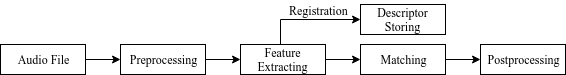
\includegraphics[scale=0.6]{pipeline.png}
    \caption{Remastered Song Identification Process}
    \label{fig:pipeline}
\end{figure}


\subsubsection{Preprocessing}
%STFT

In default audio data is represented in the time domain. Since even a small change in an audio changes the time domain representation drastically,
using the time domain representation of the audio to extract features is not recommended. Hence time domain audio signal is converted to
frequency domain signal by using \ac{stft} method. \ac{stft} is a sequence of Fourier transforms of a windowed signal\cite{Kehtarnavaz2008}.
A 2048 bits long window with 50\% overlapping was used as \ac{stft} key parameters as depicted in Figure \ref{fig:parameters}.

\begin{figure}[H]
  \centering
  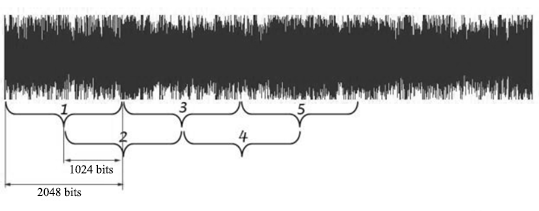
\includegraphics[scale=0.8]{parameters.png}
  \caption{Key parameters on \ac{stft}. A 2048 bits long window with 1024 bits long overlapping area.}
  \label{fig:parameters}
\end{figure}

\ac{stft} is often visualized using its spectrogram\cite{Kehtarnavaz2008}, which is an intensity plot of \ac{stft} magnitude over time. 
The generated spectrogram is converted to a color image as shown in Figure \ref{fig:spectrogram}. Axis labels and ticks are removed to stop
identification of them as key points in feature extracting step. 

\begin{figure}[H]
  \centering
  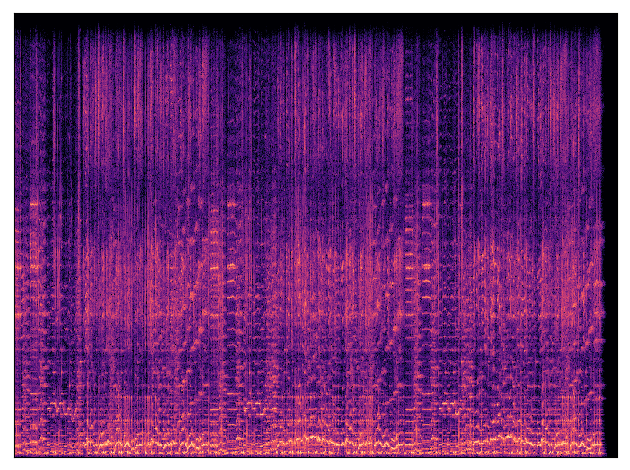
\includegraphics[scale=0.5]{spectrogram.png}
  \caption{Generated colour image of spectrogram after preprocessing.}
  \label{fig:spectrogram}
\end{figure}

\subsubsection{Feature Extracting}
%SIFT

\ac{stft} spectrogram itself can be considered as an audio descriptor\cite{Ke2005}. This method uses \ac{sift}\cite{Lowe2004} to extract 
the features which are robust to music remastering. In Figure \ref{fig:compare_spectrogram}, it can be observed that when tempo is
altered the spectrogram will either expand or compress with the time axis and when pitch is altered the spectrogram will either shift upwards or 
downwards with the frequency axis. 

\begin{figure}[H]
  \centering
  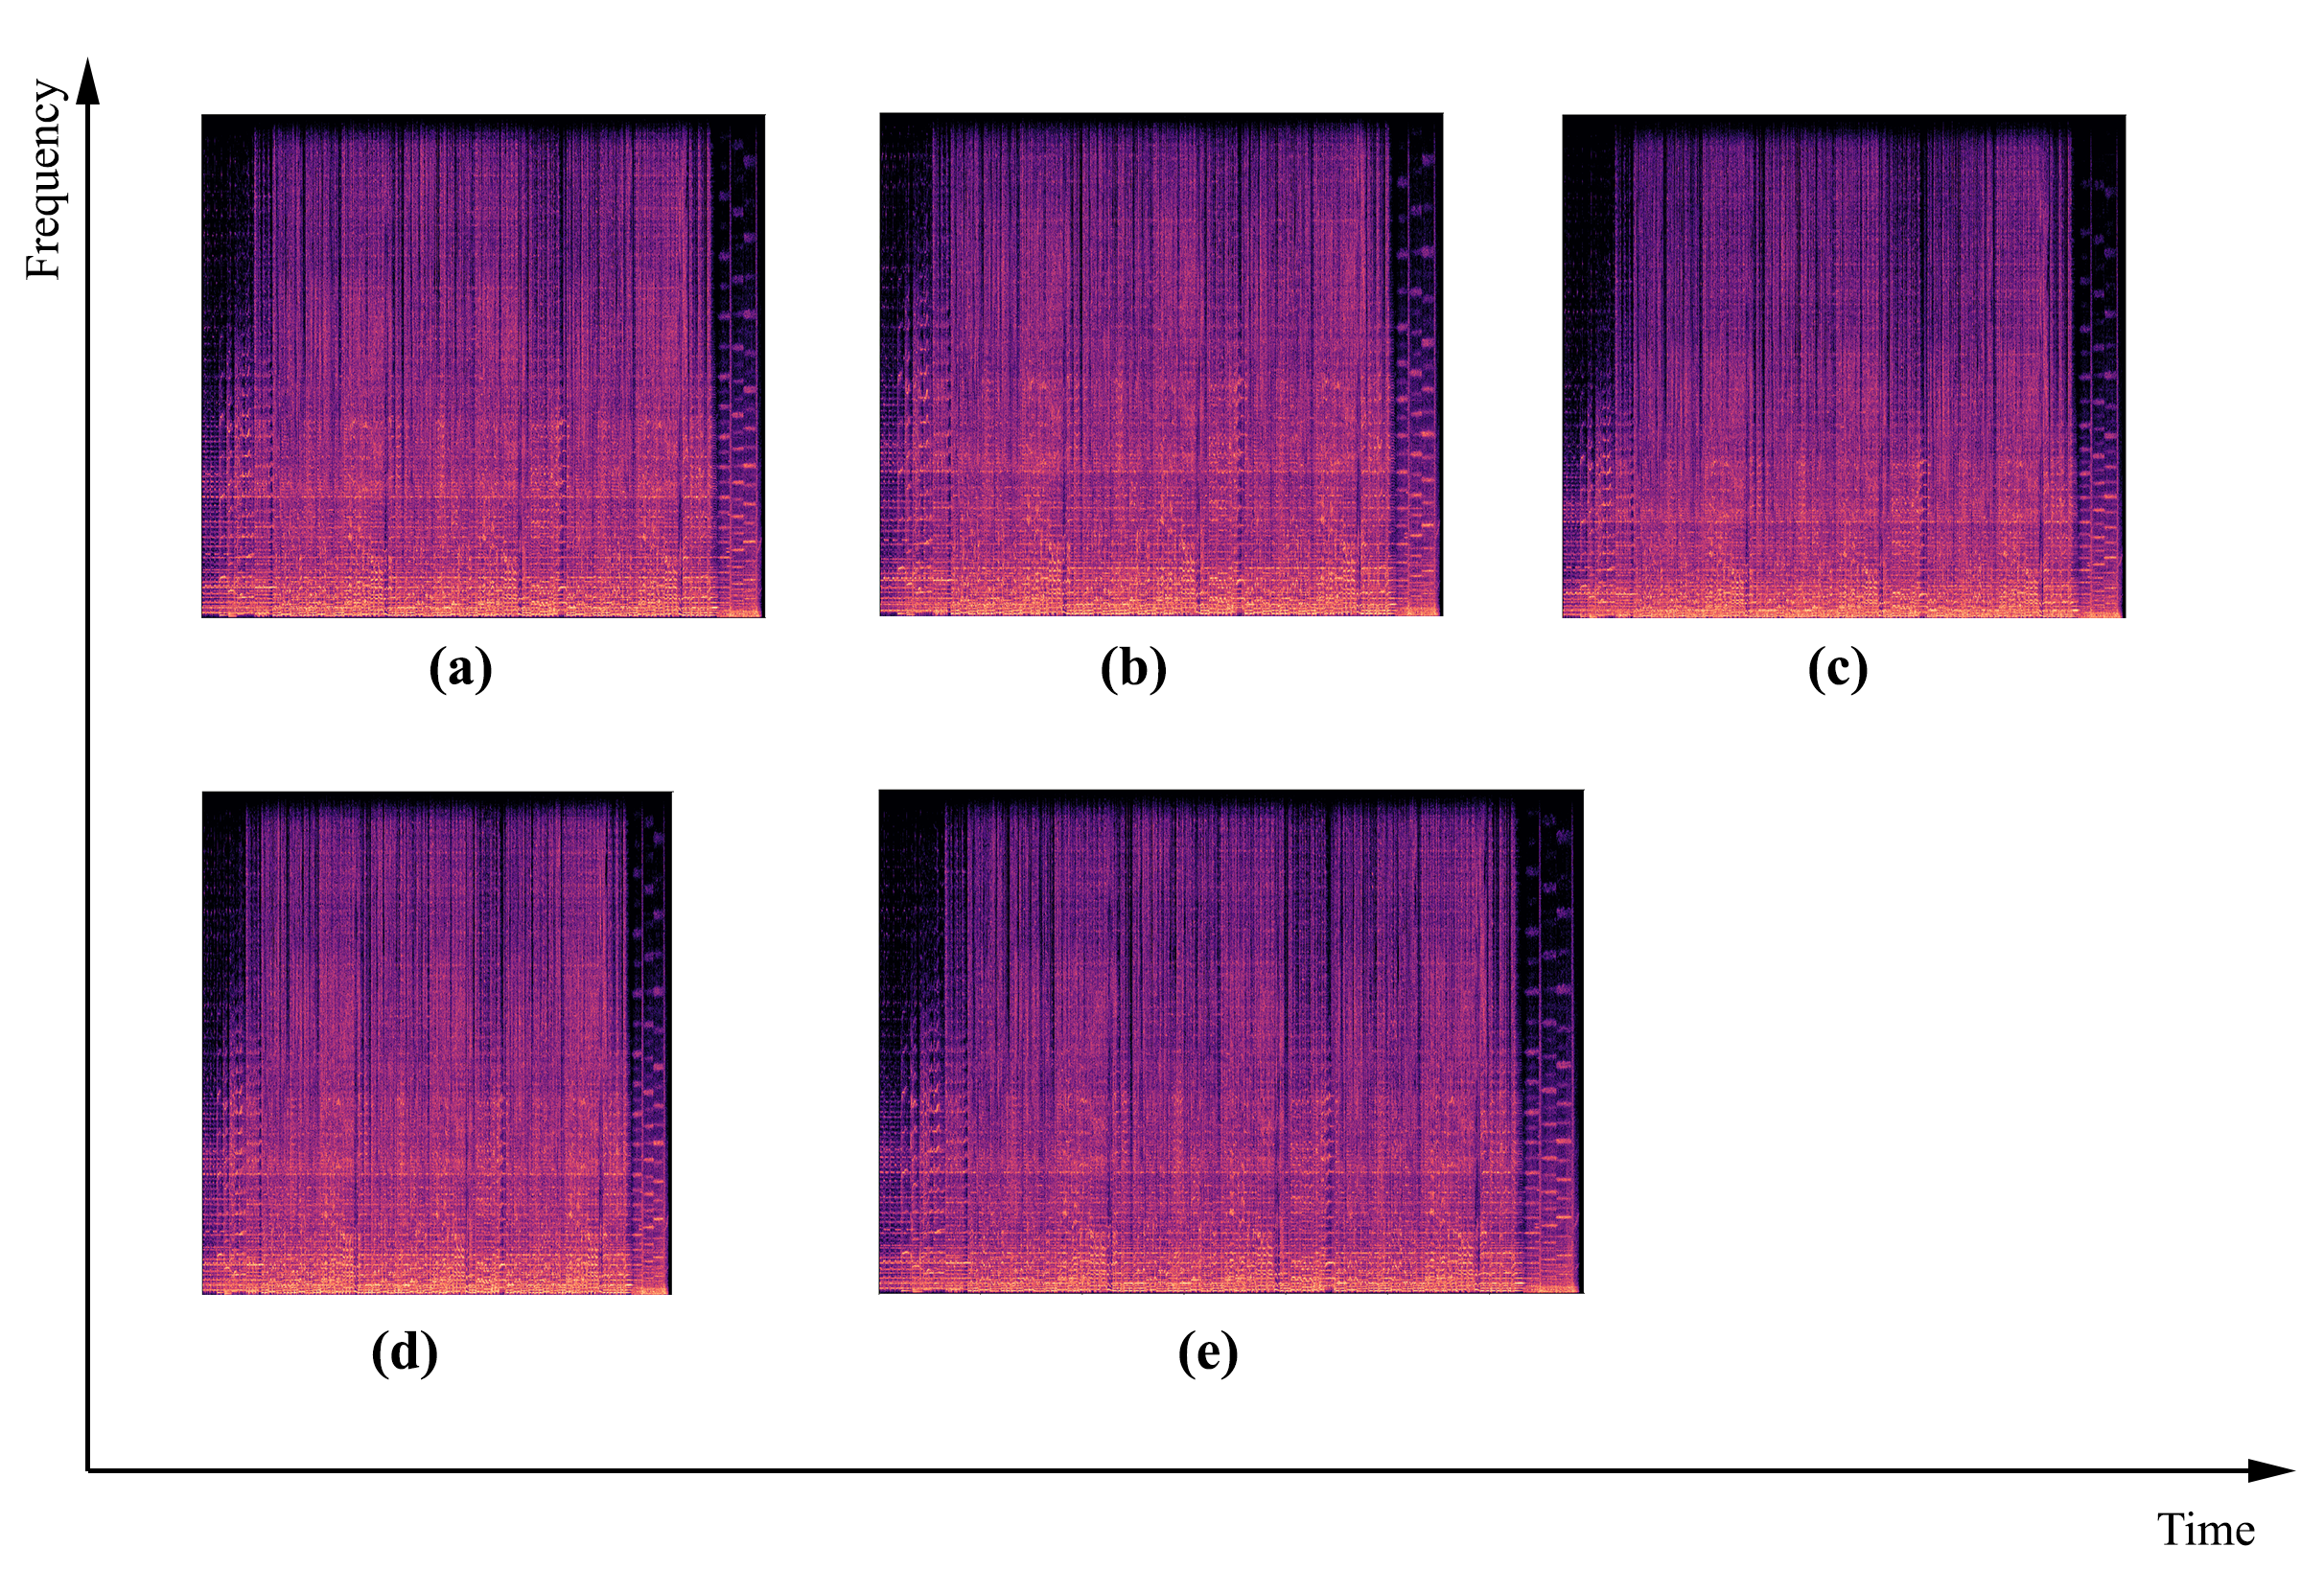
\includegraphics[scale=0.6]{spec_transform.png}
  \caption{Spectrogram transformations on audio enhancements. \textbf{(a)} is the spectrogram image of an original song. \textbf{(b)} 20\% 
  pitch increase, \textbf{(c)} 20\% pitch decrease, \textbf{(d)} 20\% tempo increase and \textbf{(e)} 20\% tempo decrease spectrogram images.}
  \label{fig:compare_spectrogram}
\end{figure}

\ac{sift} is used in computer vision to identify scale invariant features of an image. \ac{sift} features are invariant to image rotation,
scale alterations and illumination\cite{Lowe2004}. The \ac{sift} feature extractor used in this method consists of four main steps.
\begin{enumerate}
  \item Scale space extrema detection: Gaussian filters of different scales are applied to the image and potential key points are selected
  as local minima or maxima of the \ac{dog} for multiple scales.
  \item Keypoint localization: Keypoints that have low contrast or those that are poorly located along edges
  are filtered out.
  \item Orientation assignment: One or more orientations are assigned to each keypoint based on local image gradient. 
  \item Keypoint descriptor generation: Orientation histograms are created for 4 x 4 pixel neighborhoods for each keypoint.
  Each histogram consists of 8 bins, hence a (4 x 4 x 8) 128 dimensional descriptor is generated.
\end{enumerate}

A set of extracted 128 dimensional descriptors works together in describing the input audio file. Extracted 
\ac{sift} features are invariant to image stretch and translation which makes them better features to be used
in audio identification algorithm which is robust to tempo alterations and pitch shifting. 

\subsubsection{Descriptor Storing (Registering)}
\ac{sift} descriptors of original songs must be stored to use them in the matching step of the remastered
song identification process. Generally 3-5 minute music clip will have around 2000 key points in its \ac{stft}
spectrogram. Hence a \(2000\times 128\) matrix will be generated for each original song that will be registered.

The descriptor matrix of each original song is converted to a binary string and that binary string is stored 
in the database as \ac{blob}s. Converting to binary string and storing the matrix as a \ac{blob} will ensure
fast recreation of the matrix while retrieving\cite{Sears2006}.   

\subsubsection{Matching}
%Final Result
Music identification is facilitated by matching a feature matrix of a query audio clip with a feature matrix of a original song. Final goal
of the matching is to identify the count of keypoints that are matched with the original song. Identification of matching keypoints achieved
by taking 2 nearest keypoints to a query keypoint and checking whether the distance to the closest keypoint is lesser than 
the \(0.75 \times \text{distance to the 2nd closest keypoint}\).

\subsubsection{Postprocessing}
%Variable Tuning
The most similar song and matched keypoint count for a given query audio clip is identified in the matching step. But
it doesn't exactly mean that query audio clip contains that song. Because the number of keypoints that were matched
represents how much the query song matched to the most similar song. Hence there should be a threshold keypoint count
to determine whether a query audio clip contains a song in our database or not. But using just a threshold value 
won't work here since different query audio clips generate different number of key points to match against the
database. Hence ratio based threshold is recommended as a measure to determine whether the matched song is actually a
correct match. Keypoint ratio can be obtained by the below equation. 

\begin{align*}
\text{Keypoint ratio} &= \frac{\text{Matched keypoint count}}{\text{Keypoints generated for query audio clip}}\\
\end{align*}

Based on this keypoint ratio, a threshold is used to determine the validity of the match found. In order to find this
threshold value we have used 844 different audio clips with variable durations to match against 2300 original songs.
Those 844 audio clips had 519 audio clips which had songs and 325 audio clips which didn't have songs from those 
2300 original songs. And we calculated accuracy for 18 testcases which will be discussed in section 
\ref{section:experiments}, and took the average of those 18 accuracies for variable threshold values. Then results were
illustrated as shown in the Figure \ref{fig:threshold}. 

\begin{figure}[H]
  \centering
  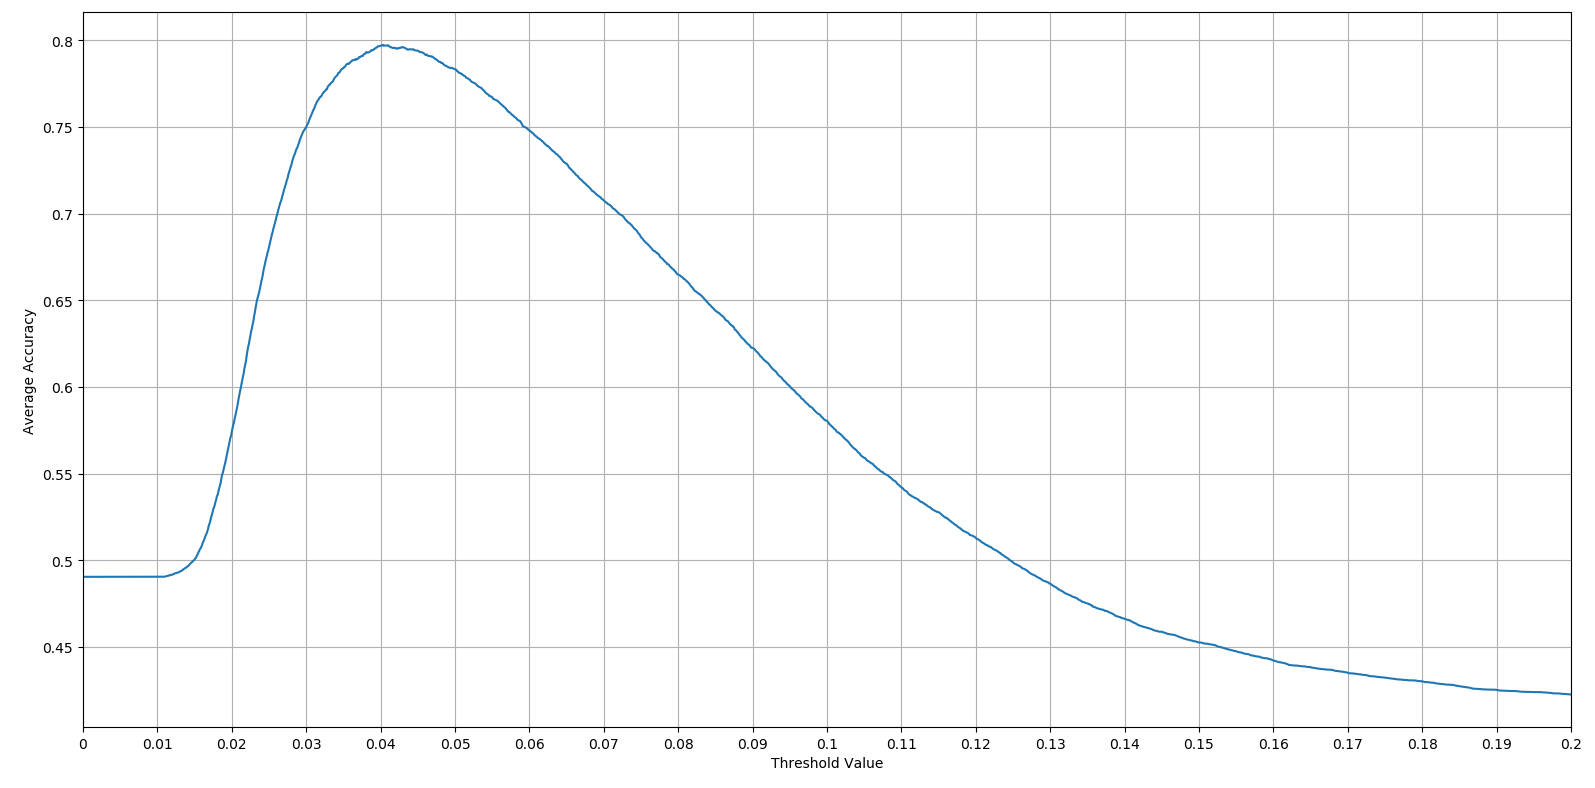
\includegraphics[scale=0.3]{threshold_adjusting.png}
  \caption{Average Accuracy Values for Different Threshold Values}
  \label{fig:threshold}
\end{figure}

Global peak can be observed in the illustration which makes that value a clear threshold point. 0.0403 is the threshold
value that was found. Hence if keypoint ratio of a query audio is larger than 0.0403 then it's identified as a valid match
to the song that was identified in the matching step, otherwise it's identified as a invalid match. This threshold point
makes this method to clearly identify whether a query audio has a song which is in a database or not.
\section{Outline of the Dissertation}

The remainder of this dissertation is organized as follows. Chapter 2 reviews the existing
related works and summarizes them. Chapter 3 describes research design and methodology while
Chapter 4 describes implementation details of the methodology. Experiments and their results
are illustrated in Chapter 5. Chapter 6, the final chapter presents the conclusion, findings
and future work. 

\clearpage
\section{Scope and Delimitations}

\subsection{In Scope}
The following areas will be covered under the research project.
\begin{itemize}
    \item Exploration of possible remastering techniques and outcomes. 
    \item Introduction of music similarity descriptor.
    \item Identification of remastered music in radio broadcasts.
\end{itemize}

\subsection{Out Scope}
The following areas will not be covered under the research project.
\begin{itemize}
    \item Identification of instrumental, acoustic or medley covers of original music. 
    \item Identification of quotations in music such as lyrical quotations or musical quotations.
\end{itemize}



\chapter{Literature Review}
\label{chapter:lit_review}
\section{Evolution of Audio}

Music has an impact on every stage of life of a human being. Audio music has been growing 
with daily life styles since prehistoric times although there isn't a particular theory 
regarding whilst and wherein music originated. Historiographers state that there are six 
periods of music and each period has a specific genre of music that vastly contributed to 
the evaluation of music upto today. In the following subsections, each music period is 
briefly described.

\subsection{Medieval Period (0-1400 A.D)}

In this period, musical notations were developed which give us an understanding of how music 
sounded at that time. The monophonic and the polyphonic were the two commonly used types of 
music during this period and most of it were subjected to religion.

\subsection{Renaissance Period (1400-1600 A.D)}

Renaissance meaning “rebirth” states a period of a new era for music where creating and perceiving 
of music were rapidly changed. Music was composed according to the new idea of concerning the thoughts 
of the listener at that time. Most of the music artists could move the listeners to devotion 
by composing music for the church.

\subsection{Baroque Period (1600-1750 A.D)}

The word “baroque” means bizzare which comes from an Italian word “Barocco”. The Baroque period is 
commonly known for complex pieces and intricate harmonies and the idea of the modern orchestra was 
created with the help of opera.

\subsection{Classical Period (1750-1800 A.D.)}

The Classical period expanded from the Baroque period making music less complex. Simpler melodies 
and forms such as the sonatas were used with the usage of the piano as the primary music instrument. 
In this era turning into public concerts is considered as a milestone in the history of music.

\subsection{Romantic Period (1800 1900 A.D.)}

Music expanded from Classical period by adding expressions and feelings with the use of various musical 
instruments such as wind instruments. Melodies were more focused on gravitating drama and emotions.

\subsection{Contemporary Period (1900-Present)}

Over time music has moved on to a complete free reign. Nowadays composers  try to do new things by 
ultimate experimentation and the usage of technology.  Music has come a long way and it has a long 
way to go and we are grateful for the countless composers who have contributed to what music is today.
\section{Audio File Formats}

Every type of digital data needs a file format to be stored in a computer 
system and the file format for digital audio data is audio file format. 
File format should be taken into consideration since audio data could vary 
from different formats in signal processing. Audio file formats can be 
categorized into three major groups.

\subsection{Uncompressed Audio Formats}

Uncompressed audio format is considered as the main type of audio format which takes a larger 
space to be stored but preserves the quality of the sound. It is vastly used on professional 
audio workstations such as the television and film industry.
Eg: WAV, AIFF, CDA


\subsection{Lossless Compressed Audio Formats}

Compared to the above type, lossless compressed audio formats take less space to be stored. 
It maintains a compression ratio of about 2:1 and reduces processing time.
Eg: FLAC, Wav Pack, Monkey’s audio, ALAC


\subsection{Lossy Compressed Audio Formats}

This type of audio formats reduce the size of the audio file which results in reducing the 
quality of sound as well. But compared to the loss of data and quality, this file format is 
used highly in limited storage capacities.
Eg: Mp3, AAC

\section{Remastered Audio Identification}

Remastered song identification falls under the domain of cover song identification,
which is a very active area of study in the \ac{mir} community \cite{SerraBook}.
Literature on cover song identification contains different approaches taken to
measure and model music similarity in both symbolic and audio domains. Literature
relevant to cover song identification can be divided into few areas such as
query-by-humming systems, content-based music retrieval, genre classification
and audio fingerprinting.

In symbolic domain of cover song identification, symbolic representations of
musical content is used in content processing. Query-by-humming systems
\cite{query_by_humming} fall under the symbolic domain as in query-by-humming
systems music contents are stored and processed in symbolic representations.
This query-by-humming method is parallel to retrieving cover songs from a song
database. Even though techniques used in query-by-humming systems could be useful
in future approaches of cover song identification, these systems can't achieve
high accuracy on real world audio music signals \cite{comparative_query_by_humming,SerraBook}.


Audio domain cover song identification approaches focus on measuring similarity
of music by exploiting music facets shared between two songs. Extracting invariant
features is used to exploit shared music facets. Although such extracted descriptors
are responsible to overcome majority of facet changes, special stress is given for
achieving tempo, key and structure since those facets are not usually managed by
the extracted descriptors themselves \cite{SerraBook}. Hence we can look at existing
literature in terms of feature extraction, tempo invariance, key invariance, structure
invariance and finally similarity comparison. Furthermore, we can take approaches which fall
into this general pipeline (refer Figure \ref{fig:general_pipeline}) to look at different techniques used for these stages and
distinguish each approach from one another by those techniques.

\begin{figure}[H]
    \centering
    \includegraphics[scale=0.5]{general_pipeline.png}
    \caption{General Pipeline for Cover Song Identification}
    \label{fig:general_pipeline}
\end{figure}

Bello's cover song identification method extracts chord sequences as the feature and
uses K transpositions for key invariance. Even though there is no technique used
for structure invariance, \ac{dp} is used for tempo invariance. Finally
it uses edit distance to compute the similarity \cite{Chord}. Since there is no technique
used for structure invariance, that method is inefficient against the structural changes
in cover songs. Egorov proposed another method which uses the same general pipeline with
extracting \ac{pcp} as the feature. But in this method Egorov uses \ac{oti} for key
invariance and \ac{dp} is used for both tempo and structural invariance. And match length
is used for similarity computation \cite{PCP}.

Foote \cite{Energy} and Izmirli \cite{KeyTemplates} introduced two methods which were using
\ac{dtw} for similarity computation and \ac{dp} for tempo invariance. Both the methods lack
techniques for key invariance and structure invariance which makes those methods to perform
inefficient in both key and temporal changes. The feature extracted by Foote is energy spectrum
while Izmirli extracted key templates. Marlot uses the same techniques for tempo invariance and
similarity computation which are \ac{dp} and \ac{dtw}, but melody is the extracted feature
which uses the key estimation for key invariance.

\begin{table}[H]
    \footnotesize
    \centering
    \begin{tabular}{|l|c|c|c|c|c|}
        \hline
        \multicolumn{1}{|c|}{\textbf{Research}} & \textbf{Feature}                   & \textbf{\begin{tabular}[c]{@{}c@{}}Key \\ Invariance\end{tabular}}  & \textbf{\begin{tabular}[c]{@{}c@{}}Tempo\\ Invariance\end{tabular}} & \textbf{\begin{tabular}[c]{@{}c@{}}Structure\\ Invariance\end{tabular}} & \textbf{\begin{tabular}[c]{@{}c@{}}Similarity\\ Computation\end{tabular}} \\[2ex] \hline
        \textbf{Bello \cite{Chord}}             & \textbf{Chords}                     & \textbf{\begin{tabular}[c]{@{}c@{}}K\\ transpositions\end{tabular}}  & \textbf{DP}                        & \textbf{ - }                          & \textbf{\begin{tabular}[c]{@{}c@{}}Edit\\ distance\end{tabular}} \\[2ex] \hline
        \textbf{\begin{tabular}[c]{@{}l@{}}Egorov \& \\ Linetsky \cite{PCP}\end{tabular}}      & \textbf{PCP}                        & \textbf{OTI}                        & \textbf{DP}                        & \textbf{DP}                        & \textbf{\begin{tabular}[c]{@{}c@{}}Match\\ length\end{tabular}} \\[2ex] \hline
        \textbf{Foote \cite{Energy}}            & \textbf{\begin{tabular}[c]{@{}c@{}}Energy \\ spectral\end{tabular}} & \textbf{-}                           & \textbf{DP}                        & \textbf{ - }                          & \textbf{DTW}                       \\[2ex] \hline
        \textbf{Izmiril \cite{KeyTemplates}}    & \textbf{\begin{tabular}[c]{@{}c@{}}Key \\ templates\end{tabular}} & \textbf{-}                           & \textbf{DP}                        & \textbf{ - }                          & \textbf{DTW}                       \\[2ex] \hline
        \textbf{Marolt \cite{Melody}}           & \textbf{Melody}                     & \textbf{\begin{tabular}[c]{@{}c@{}}Key \\ estimation\end{tabular}} & \textbf{DP}                        & \textbf{ - }                          & \textbf{DTW}                       \\[2ex] \hline
    \end{tabular}
    \caption{Cover song identification methods and their techniques used for each step in general pipeline}
    \label{tab:literature}
\end{table}

Related works mentioned above for audio domain can be modelled to the general pipeline for cover
song identification (refer Figure \ref{fig:general_pipeline}) as described in Table \ref{tab:literature}.


\chapter{Design}
\label{chapter:design}
\section{Architectural Design}

The basic framework to identify music in radio broadcasts is proposed in 
\say{Radio Broadcast Monitoring to Ensure Copyright Ownership}\cite{Nishan}. And it's currently
implemented and deployed in \ac{osca}. Hence the infrastructure to contain the basic framework
of a radio monitoring system is already there. When different methods of music identification
are applied to radio broadcast monitoring, only registering service, database and matching service
will be changed conserving the other modules that are in the architecture as shown in the Figure
\ref{fig:new_arch}.

\begin{figure}[H]
    \centering
    \includegraphics[scale=0.6]{NewSystem.png}
    \caption{Architectural Design}
    \label{fig:new_arch}
\end{figure}

Registering service takes original songs as input and generates specific descriptors to be stored
in the database. Database stores the generated audio descriptors by the registering service in a
retrieval friendly framework to help the matching service to retrieve descriptors faster. The matching
service takes a query audio clip and determines whether that query audio clip contains a song registered
before.     
\clearpage
\section{Principle Component Analysis (PCA)}
There are many different approaches to identify music by extracting different audio features as
discussed in the Chapter \ref{chapter:lit_review}. Since there are very low number of researches
conducted on sinhala music identification, finding audio features which can differentiate two 
sinhala songs was required to continue the research. Hence \ac{pca} was conducted to find features
on a 5000 song dataset extracting 27 different audio features and results were collected for 
different normalization techniques. \ac{svd} was used to composite multi-dimension features.

\subsection{PCA with Raw Dataset}

Initially a \ac{pca} was executed on the raw feature matrix without any normalization technique
which led to the results in Figure \ref{fig:pca_coeff}. Abnormality of the result caused to 
revisit the feature matrix and need of a normalization technique was identified. 

\begin{figure}[H]
    \centering
    \includegraphics[scale=0.35]{pca_coeff.png}
    \caption{PCA coefficients weighted by eigen values}
    \label{fig:pca_coeff}
\end{figure}

\subsection{PCA with Dataset Normalized by Z-score}

Then \ac{pca} was conducted on the dataset which was normalized by z-score which produced results
on Figure \ref{fig:pca_coeff_z}. While analyzing the results, it was observed that results
indicate uniform variance among the features that was not present in the original feature
matrix. Hence need of a normalization technique which preserve the variance of a feature was
identified. 

\begin{figure}[H]
    \centering
    \includegraphics[scale=0.35]{pca_coeff_z.png}
    \caption{PCA coefficients weighted by eigen values (Normalized by Zscore)}
    \label{fig:pca_coeff_z}
\end{figure}

\subsection{PCA with Dataset Normalized by Rescaling}

Finally the dataset was normalized by rescaling and the conducted \ac{pca} gave a justifiable result
which is shown in Figure \ref{fig:pca_coeff_z}. \say{Area Method of Moments} and \say{Area 
Method of Moments of MFCCs} are identified as the two features which covers majority of the variance
in the dataset. 

\begin{figure}[H]
    \centering
    \includegraphics[scale=0.35]{pca_coeff_re.png}
    \caption{PCA coefficients weighted by eigen values (Normalized by Rescaling)}
    \label{fig:pca_coeff_re}
\end{figure}

Then those two features were extracted from audio clips with slight changes to tempo and pitch, in order 
to check whether those two features show any invariance to pitch or the tempo. But when tempo or pitch changed
slightly, \ac{svd} values of those features changed drastically. Therefore results of the \ac{pca} couldn't
be used to progress on this research which resulted to revisit the literature to find better features to 
extract. 
\section{Scale Invariant Feature Transform (SIFT) Based Approach}

\ac{sift} is a method of extracting features from a image which are invariant 
to scale modifications\cite{Lowe2004}. Approaching music identification with
image processing techniques found in literature as discussed in Chapter \ref{chapter:lit_review}.
Pitch shifting can be identified as an expansion or a compression of the \ac{stft}
spectrogram over the frequency axis, while tempo alterations can be identified 
as an expansion or a compression over the time axis as depicted in Figure \ref{fig:compare_spectrogram_design}.
Hence \ac{sift} can be used to find similarity of a tempo altered or pitch altered audio
using it's \ac{stft} spectrogram. 

\begin{figure}[h]
    \centering
    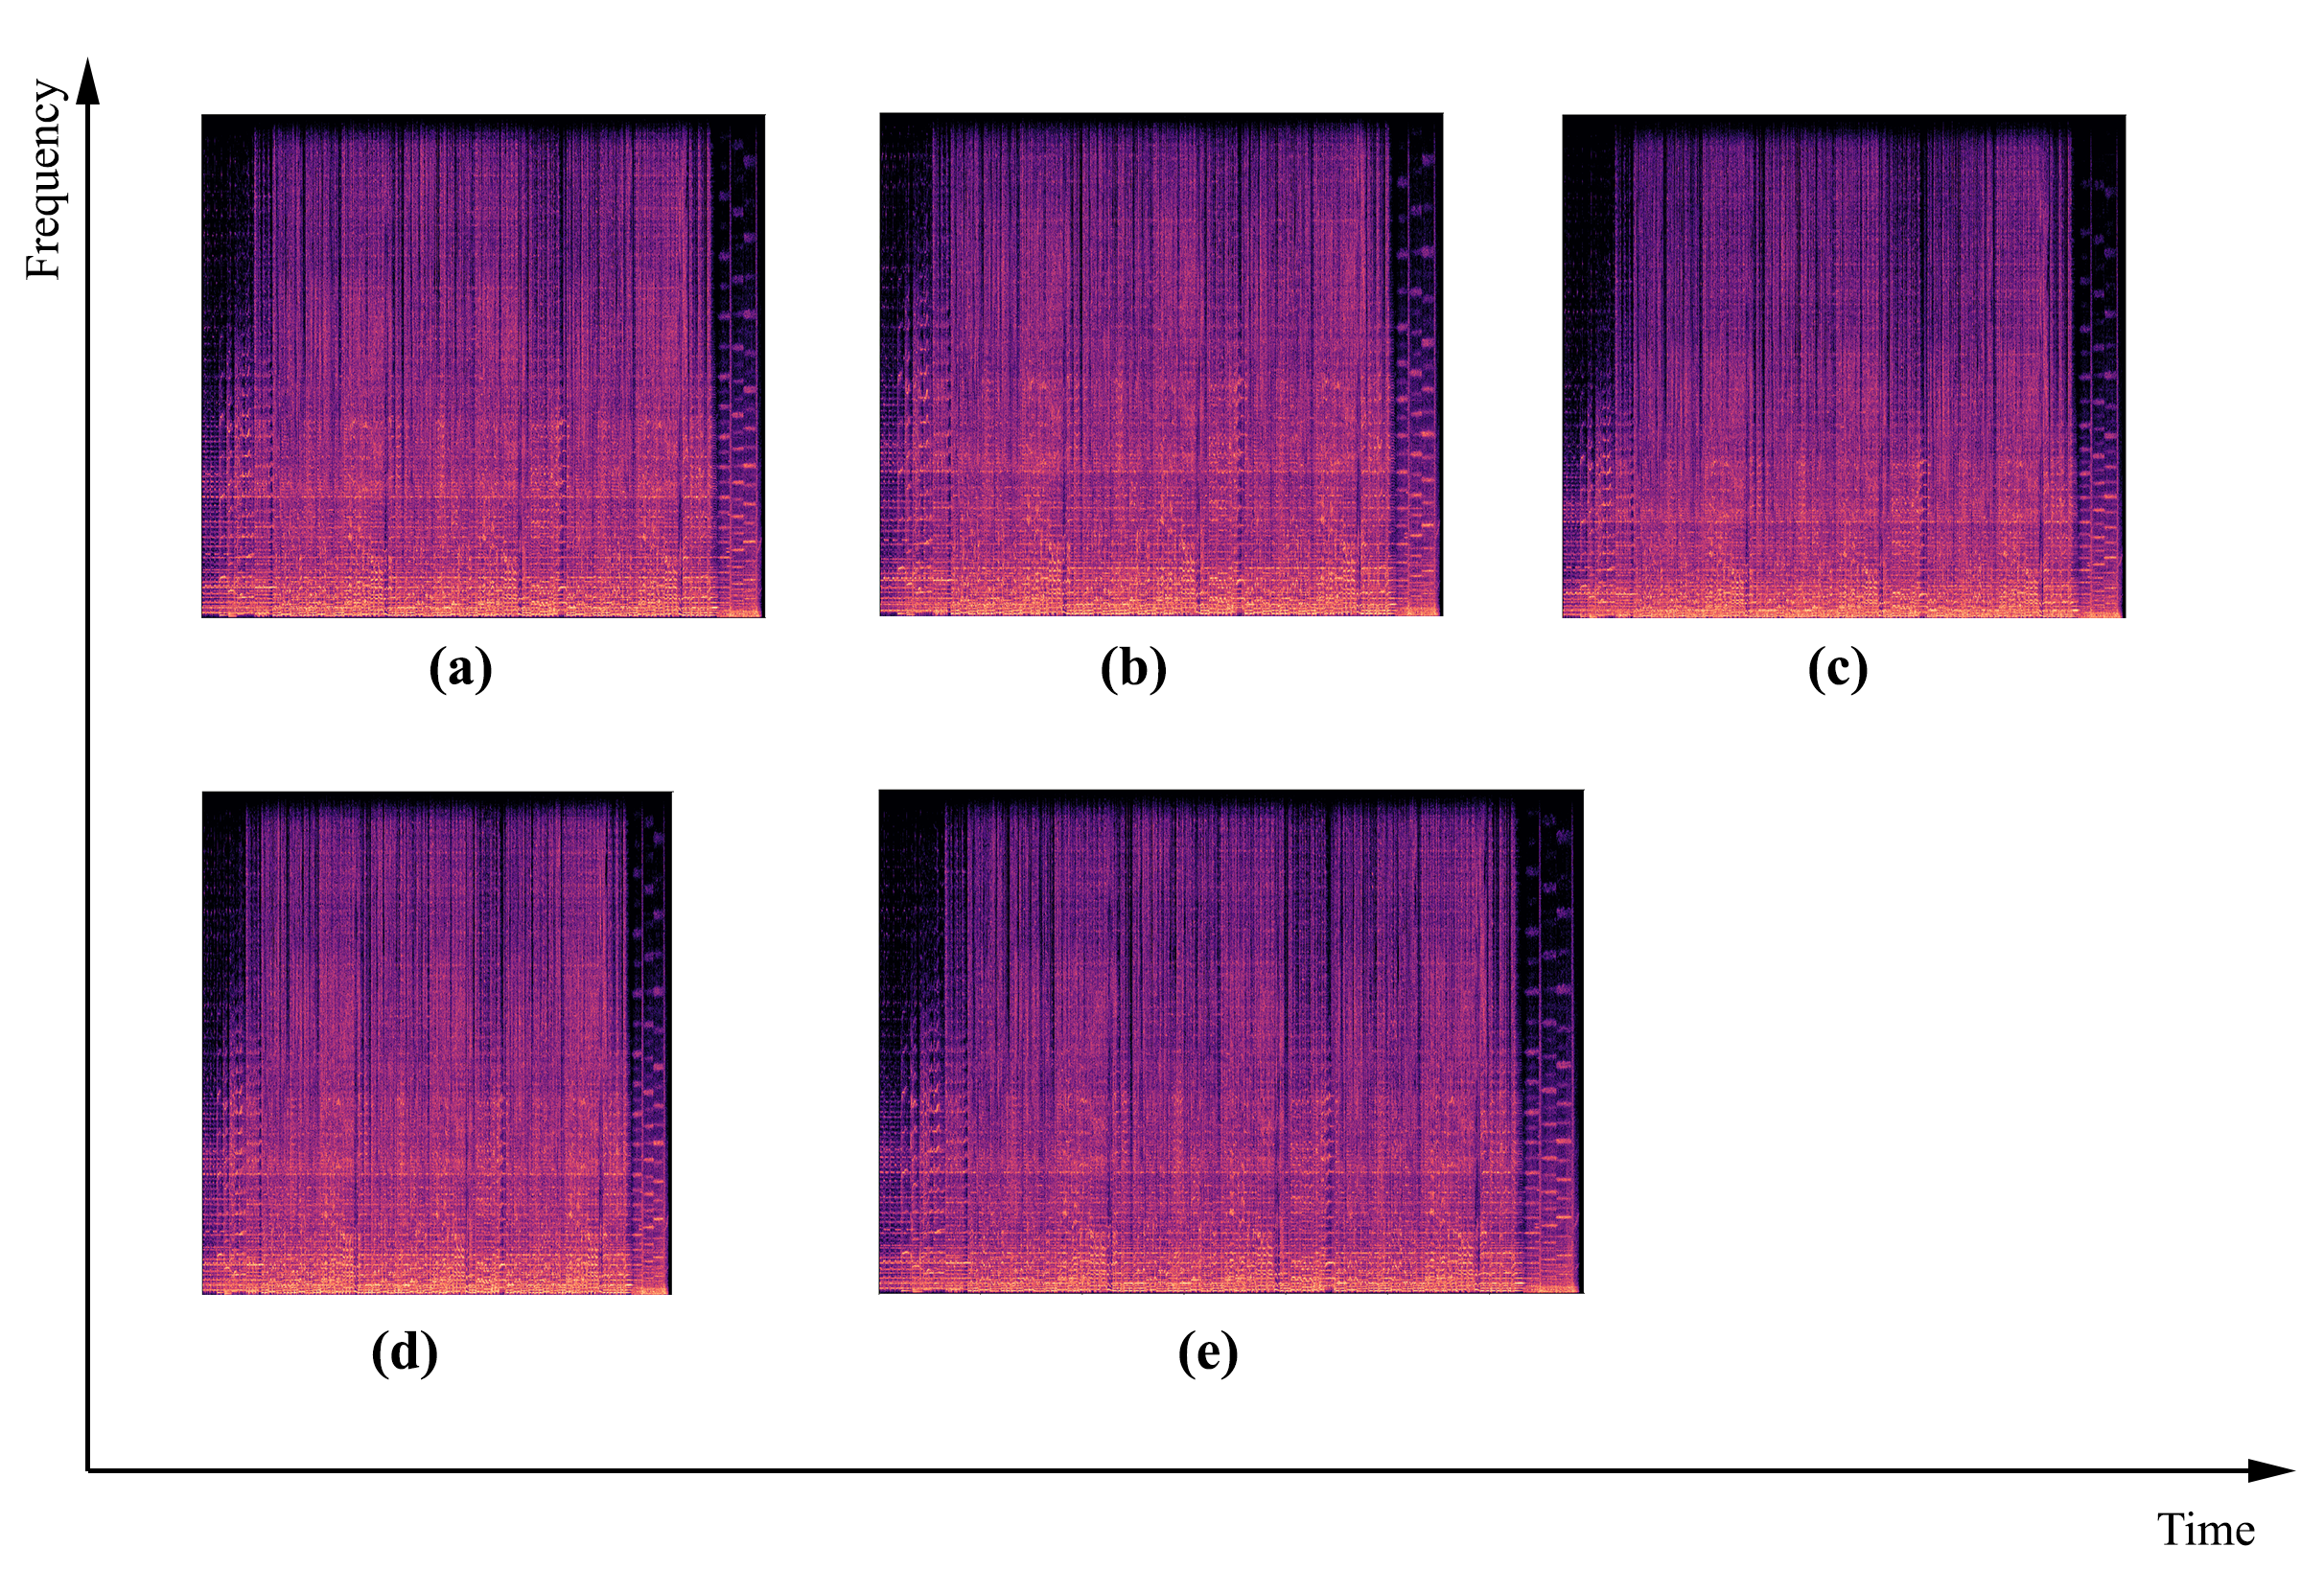
\includegraphics[scale=0.6]{spec_transform.png}
    \caption{Spectrogram transformations on audio enhancements. \textbf{(a)} is the spectrogram image of a original song. \textbf{(b)} 20\% 
    pitch increase, \textbf{(c)} 20\% pitch decrease, \textbf{(d)} 20\% tempo increase and \textbf{(e)} 20\% tempo decrease spectrogram images.}
    \label{fig:compare_spectrogram_design}
  \end{figure}

\subsection{Short Time Fourier Transform}

\ac{stft}\cite{Kehtarnavaz2008} is used to transform a signal from time domain to frequency domain as time domain signals
are unstable. When selecting key parameters 2048 bits long window was used with 50\% overlap as depicted in Figure 
\ref{fig:spectrogram_parameters}, in order to ensure that every part of a signal is represented in two windows.

\begin{figure}[H]
    \centering
    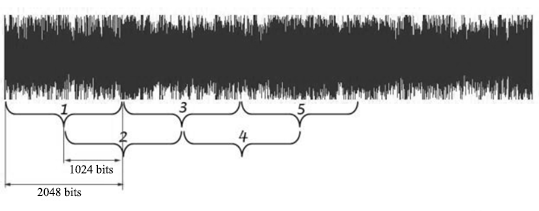
\includegraphics[scale=0.8]{parameters.png}
    \caption{Key parameters on \ac{stft}. 2048 bits long window with 1024 bits long overlapping area.}
    \label{fig:spectrogram_parameters}
  \end{figure}

  \ac{stft} is often visualized using its spectrogram\cite{Kehtarnavaz2008}, which is an intensity plot of \ac{stft} magnitude over time. 
  The generated spectrogram is converted to a color image as shown in Figure \ref{fig:spectrogram_design}. Axis labels and ticks are removed to stop
  identification of them as key points in feature extracting step. 

  \begin{figure}[H]
    \centering
    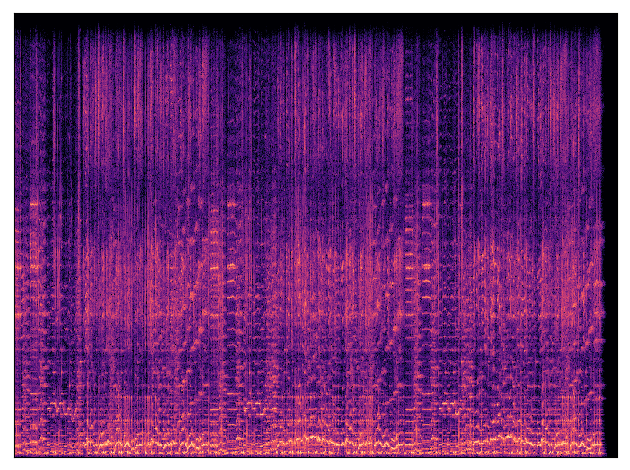
\includegraphics[scale=0.5]{spectrogram.png}
    \caption{Generated colour image of a spectrogram}
    \label{fig:spectrogram_design}
  \end{figure}

\subsection{SIFT Descriptor Extraction}

\ac{sift} is used in computer vision to identify scale invariant features of an image. \ac{sift} features are invariant to image rotation,
scale alterations and illumination\cite{Lowe2004}. The \ac{sift} feature extractor used in this method consists of four main steps.
\begin{enumerate}
  \item Scale space extrema detection: Gaussian filters of different scales are applied to the image and potential key points are selected
  as local minima or maxima of the \ac{dog} for multiple scales.
  \item Keypoint localization: Keypoints that have low contrast or those that are poorly located along edges
  are filtered out.
  \item Orientation assignment: One or more orientations are assigned to each keypoint based on local image gradient. 
  \item Keypoint descriptor generation: Orientation histograms are created for 4 x 4 pixel neighborhoods for each keypoint.
  Each histogram consists 8 bins, hence (4 x 4 x 8) 128 dimensional descriptor is generated.
\end{enumerate}

\ac{sift} generate (\(\text{No of Keypoints} \times 128\)) dimension matrix for each spectrogram. In average, more than 1000 keypoints 
are identified from a single spectrogram as shown in the Figure \ref{fig:spectrogram_keypoints}.  

  \begin{figure}[H]
    \centering
    \includegraphics[scale=0.5]{sift_keypoints.jpg}
    \caption{Identified keypoints in a SIFT spectrogram}
    \label{fig:spectrogram_keypoints}
  \end{figure}

\subsection{SIFT Descriptor Matching}

Music identification is facilitated by matching a feature matrix of a query audio clip with a feature matrix of a original song. Final goal
of the matching is to identify the count of keypoints that are matched with the original song. Identification of matching keypoints achieved
by taking 2 nearest keypoints to a query keypoint and checking whether the distance to the closest keypoint is lesser than 
the \(0.75 \times \text{distance to the 2nd closest keypoint}\). Those keypoints which were matched can be visualized as shown in the 
Figure \ref{fig:spectrogram_match}.

\begin{figure}[H]
    \centering
    \includegraphics[scale=0.3]{spec_match.png}
    \caption{Matched keypoints of two spectrograms}
    \label{fig:spectrogram_match}
  \end{figure}

\subsection{Thresholding}

Final step is to determine whether that query audio clip has the matched original song or not. It's archived by a thresholding method. 
In the begging keypoint count was used as the threshold measure. But it had drawbacks such as when query audio is variable length
number of keypoints identified will be different which eventually leads to different number of keypoints matched. Hence just using
keypoint count as a threshold measure didn't work as finding a generalized threshold value is really different. 

Therefore a ratio based threshold measure was recommended. Where we consider both number of keypoints that matched and initially identified 
keypoints count. Keypoint ratio can be obtained by below equation.

\begin{align*}
    \text{Keypoint ratio} &= \frac{\text{Matched keypoint count}}{\text{Keypoints generated for query audio clip}}\\
\end{align*}

Keypoint ratio can be used as better threshold measure as we can find generalized threshold value irrespective of length of the query audio clip. 
Threshold value selection and results will be discussed on Section \ref{section:results}. 

\chapter{Implementation}
\section{Principle Component Analysis (PCA)}

\subsection{Dataset}

Song dataset with 5000 songs were obtained from the \ac{osca} as mp3 files with 320kbps quality. Then
those 5000 songs were converted to wav format with 16-pcm quality by using ffmpeg library.

\subsection{Features and Tools}

Jaudio library\cite{jaudio} was used to extract 27 different audio features from the song dataset.
Then \ac{svd} function in Matlab\cite{matlab:2018b} was used to composite multi-dimension features
to a single value. Finally \ac{pca} implementation in Matlab\cite{matlab:2018b} used to run the \ac{pca}. 
\section{Scale Invariant Feature Transform (SIFT) Based Approach}

\subsection{Short Time Fourier Transform}
\ac{stft} implementation of librosa\cite{librosa} library used to get the
\ac{stft} spectrogram of the audio signal. Parameters given to off both axis bars
on generated \ac{stft} spectrogram as spectrogram needed to be isolated.  

\subsection{SIFT Descriptor Extraction and Matching}
OpenCV\cite{opencv} \ac{sift} implementation was used to identify keypoints and
generate \ac{sift} descriptors. Brute-force matcher implementation on OpenCV\cite{opencv} was the matcher used 
to match two \ac{sift} feature vectors. 



\chapter{Results and Evaluation}
\section{Experiments}
\label{section:experiments}

%song dataset
\subsection{Song Dataset}
A song dataset consisting 2300 sinhala songs were used in the registration step of the experiment. These 2300 sinhala songs were retrieved from
\ac{osca} of Sri Lanka which works as the governing organization to ensure intellectual property rights of music in Sri Lanka. 

%query audio samples
\subsection{Query Audio Samples}
Variable sized 844 query audio clips were used for the experiment to evaluate the performance of this method
against different durations. 519 of the above mentioned audio clips had songs which are in the database while 325 audio clips didn't have songs from 
the database. Hence for each test case, the sample size was 844 query audio clips with 0.61492 prevalence.    

%test cases
\subsection{Test Cases}
Test cases were created by doing audio distortions to the query audio samples. Performance of the method was evaluated for three main audio distortions
which are tempo alteration, pitch alteration and both pitch and tempo alteration. Both increased and decreased alterations are considered for three different
levels of alterations which are 10\% alteration, 20\% alteration and 50\% alteration. Hence there are 3 audio distortions, 2 audio distortion directions and
3 audio alteration levels, 18 (\(3 \times 2 \times 3\)) test cases were generated to evaluate the performance. 



\clearpage
%test results
\section{Experiment Results}
\label{section:results}

The proposed method has an exact way to identify whether a query audio clip has a matching registered song or not. Therefore this method can be considered as
a classifier. A classifier can be evaluated by the confusion matrix generated for a given sample. \ac{tp}, \ac{fp}, \ac{tn} and \ac{fn} were calculated
for each test case. Then accuracy and \ac{fp} rate was calculated for each test case. Reducing \ac{fp} rate is significant as much as increasing the accuracy
given that this method mainly focuses on identifying music on radio broadcasts. Accuracy and \ac{fp} rate can be calculated from the formulas given below. 

\begin{align*}
    \text{Accuracy} &= \frac{TP+TN}{TP+TN+FP+FN}\\
    \\
    \text{FP Rate} &= \frac{FP}{FP+TN}\\
\end{align*}

Keypoint ratio based threshold is proposed as the threshold measure in this method. Two experiments were done, one with keypoint count as threshold measure and the
other with keypoint ratio as threshold measure to validate the claim of keypoint ratio is better threshold measure. 

\subsection{Using Keypoint Count as Threshold}

Average accuracies for different threshold values are illustrated as shown in Figure \ref{fig:threshold_old} to identify the optimal threshold value to use. Since
the visualization clearly indicates a global peak value which is keypoint count of 69, that value can be used as the threshold value. This threshold value of 69 is
used in this experiment. 
\vspace{12pt}

Results of the experiment using keypoint count as the threshold measure are presented in Table \ref{tab:test_results_keypoint}. There is no clear
change between accuracies of pitch changes and tempo changes when using keypoint count as the threshold measure. Pitch changes and tempo changes
up to 20\% alteration can be identified with 92\%-98\% accuracy. 


\begin{figure}[H]
    \centering
    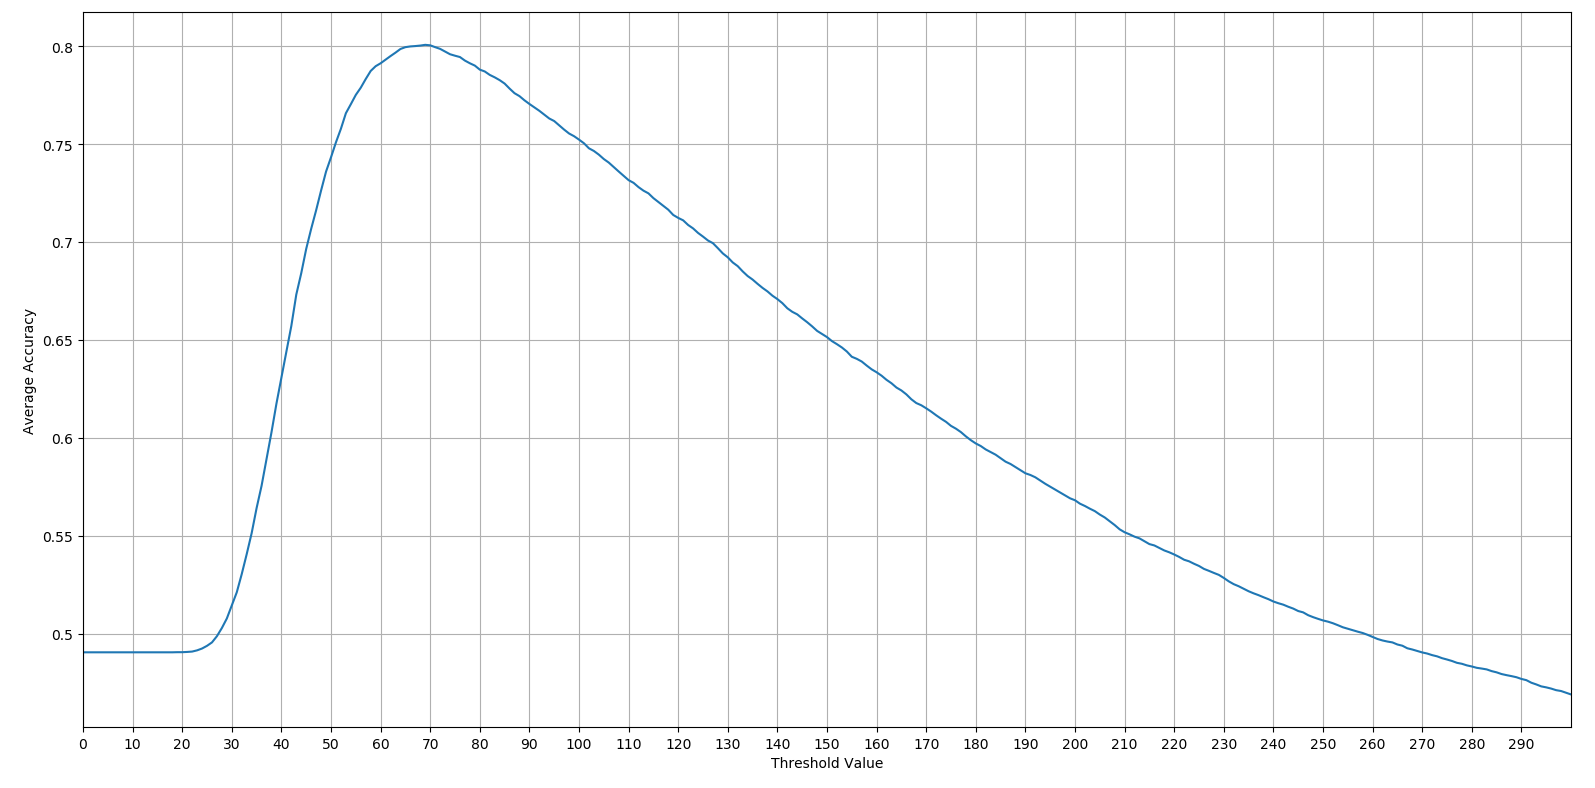
\includegraphics[scale=0.3]{threshold_adjusting_old.png}
    \caption{Average Accuracy Values for Different Threshold Values (Keypoint Count)}
    \label{fig:threshold_old}
  \end{figure}
  


\begin{table}[H]
    \begin{tabular}{|l|r|r|r|r|r|r|}
        \hline
        \textbf{Test Case}                  & \textbf{TP}   & \textbf{FP} & \textbf{TN} & \textbf{FN} & \textbf{Accuracy} & \textbf{FP Rate} \\ \hline
        Tempo Increase 10\%                & 509         & 19          & 306         & 10          & 0.96564           & 0.05846          \\ \hline
        Tempo Increase 20\%                & 509         & 18          & 307         & 10          & 0.96682           & 0.05538          \\ \hline
        Tempo Increase 50\%                & 497         & 10          & 315         & 22          & 0.96209           & 0.03077          \\ \hline
        Tempo Decrease 10\%                & 515         & 16          & 309         & 4           & 0.97630           & 0.04923          \\ \hline
        Tempo Decrease 20\%                & 516         & 19          & 306         & 3           & 0.97393           & 0.05846          \\ \hline
        Tempo Decrease 50\%                & 517         & 22          & 303         & 2           & 0.97156           & 0.06769          \\ \hline
        Pitch Increase 10\%                & 514         & 21          & 304         & 5           & 0.96919           & 0.06462          \\ \hline
        Pitch Increase 20\%                & 513         & 11          & 314         & 6           & 0.97986           & 0.03385          \\ \hline
        Pitch Increase 50\%                & 7           & 27          & 298         & 512         & 0.36137           & 0.08308          \\ \hline
        Pitch Decrease 10\%                & 511         & 11          & 314         & 8           & 0.97749           & 0.03385          \\ \hline
        Pitch Decrease 20\%                & 463         & 4           & 321         & 56          & 0.92891           & 0.01231          \\ \hline
        Pitch Decrease 50\%                & 0           & 0           & 325         & 519         & 0.38507           & 0.00000          \\ \hline
        Tempo \& Pitch Increase 10\%       & 414         & 11          & 314         & 105         & 0.86256           & 0.03385          \\ \hline
        Tempo \& Pitch Increase 20\%       & 339         & 18          & 307         & 180         & 0.76540           & 0.05538          \\ \hline
        Tempo \& Pitch Increase 50\%       & 0           & 26          & 299         & 519         & 0.35427           & 0.08000          \\ \hline
        Tempo \& Pitch Decrease 10\%       & 373         & 5           & 320         & 146         & 0.82109           & 0.01538          \\ \hline
        Tempo \& Pitch Decrease 20\%       & 226         & 2           & 323         & 293         & 0.65047           & 0.00615          \\ \hline
        Tempo \& Pitch Decrease 50\%       & 0           & 0           & 325         & 519         & 0.38507           & 0.00000          \\ \hline
    \end{tabular}
    \caption{Experiment results using keypoint count as threshold}
    \label{tab:test_results_keypoint}
\end{table}


\subsection{Using Keypoint Ratio as Threshold}

Average accuracies for different threshold values are illustrated as shown in Figure \ref{fig:threshold_new} to identify the optimal threshold value to use. Since
the visualization clearly indicates a global peak value which is keypoint count of 0.0403, that value can be used as the threshold value. This threshold value of 
0.0403 is used in this experiment. 
\vspace{12pt}

Results of the experiment using keypoint ratio as the threshold measure presented in Table \ref{tab:test_results_keypoint_ratio}. It can be observed that accuracies
have increased considerably compared to results of the experiment which uses keypoint count as the threshold measure which validates the claim of taking keypoint ratio as
a better threshold measure. Pitch changes and tempo changes up to 20\% alteration can be identified with 95\%-99\% accuracy.

\begin{figure}[H]
    \centering
    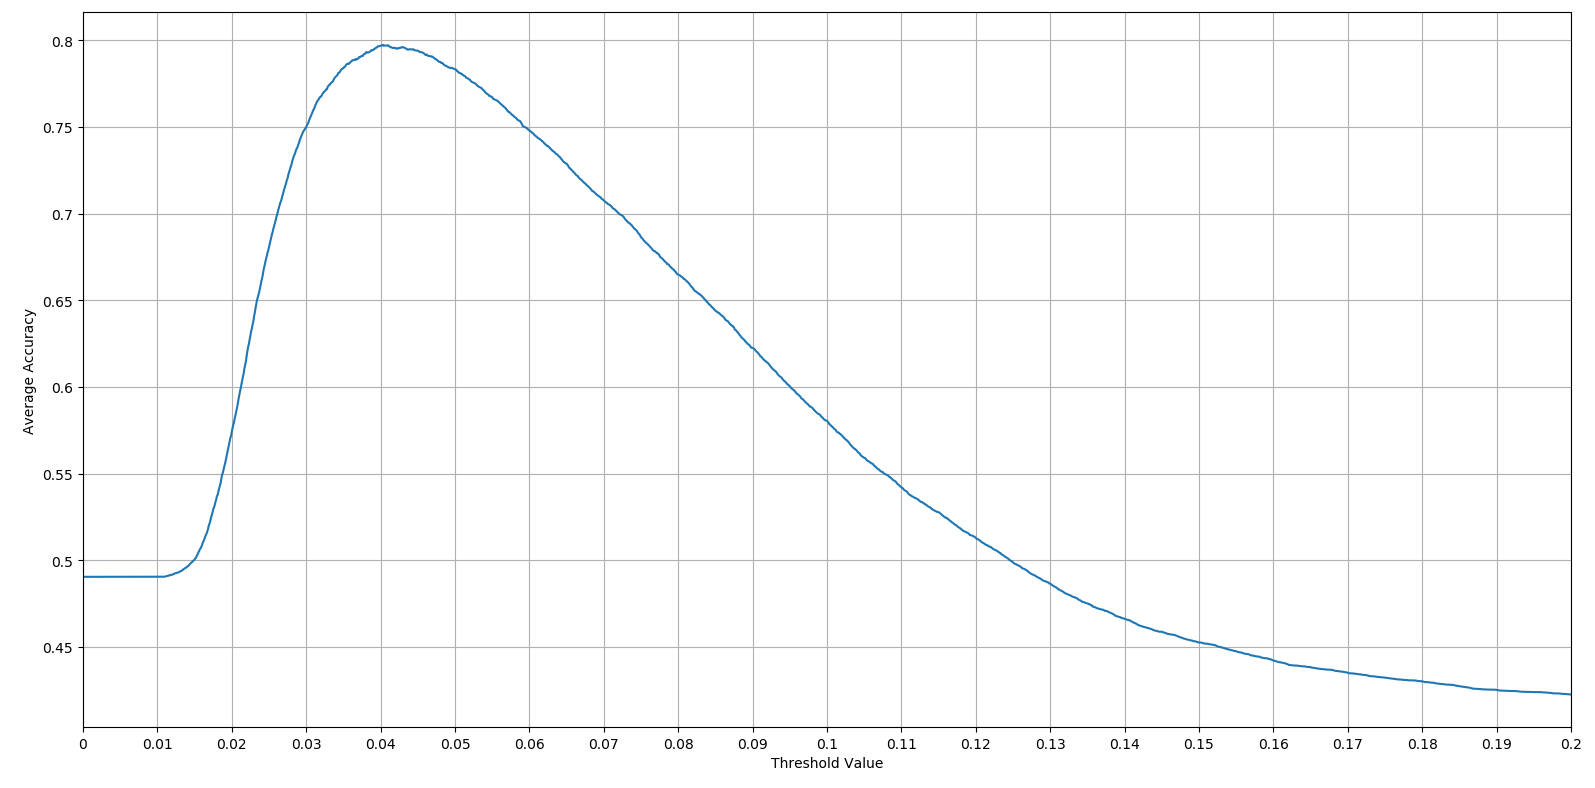
\includegraphics[scale=0.3]{threshold_adjusting.png}
    \caption{Average Accuracy Values for Different Threshold Values (Keypoint Ratio)}
    \label{fig:threshold_new}
  \end{figure}

\begin{table}[H]
    \begin{tabular}{|l|r|r|r|r|r|r|}
        \hline
        \textbf{Test Case}                 & \textbf{TP}   & \textbf{FP} & \textbf{TN} & \textbf{FN} & \textbf{Accuracy} & \textbf{FP Rate} \\ \hline
        Tempo Increase 10\%                & 512         & 13          & 312         & 7           & 0.97630           & 0.04000          \\ \hline
        Tempo Increase 20\%                & 508         & 10          & 315         & 11          & 0.97512           & 0.03077          \\ \hline
        Tempo Increase 50\%                & 501         & 9           & 316         & 18          & 0.96801           & 0.02769          \\ \hline
        Tempo Decrease 10\%                & 515         & 11          & 314         & 4           & 0.98223           & 0.03385          \\ \hline
        Tempo Decrease 20\%                & 519         & 10          & 315         & 0           & 0.98815           & 0.03077          \\ \hline
        Tempo Decrease 50\%                & 519         & 9           & 316         & 0           & 0.98934           & 0.02769          \\ \hline
        Pitch Increase 10\%                & 519         & 9           & 316         & 0           & 0.98934           & 0.02769          \\ \hline
        Pitch Increase 20\%                & 517         & 9           & 316         & 2           & 0.98697           & 0.02769          \\ \hline
        Pitch Increase 50\%                & 0           & 4           & 321         & 519         & 0.38033           & 0.01231          \\ \hline
        Pitch Decrease 10\%                & 516         & 16          & 309         & 3           & 0.97749           & 0.04923          \\ \hline
        Pitch Decrease 20\%                & 503         & 25          & 300         & 16          & 0.95142           & 0.07692          \\ \hline
        Pitch Decrease 50\%                & 23          & 160         & 165         & 496         & 0.22275           & 0.49231          \\ \hline
        Tempo  \& Pitch Increase 10\%      & 413         & 11          & 314         & 106         & 0.86137           & 0.03385          \\ \hline
        Tempo  \& Pitch Increase 20\% & 287         & 17          & 308         & 232         & 0.70498           & 0.05231          \\ \hline
        Tempo  \& Pitch Increase 50\% & 0           & 7           & 318         & 519         & 0.37678           & 0.02154          \\ \hline
        Tempo  \& Pitch Decrease 10\% & 432         & 28          & 297         & 87          & 0.86374           & 0.08615          \\ \hline
        Tempo  \& Pitch Decrease 20\% & 346         & 34          & 291         & 173         & 0.75474           & 0.10462          \\ \hline
        Tempo  \& Pitch Decrease 50\% & 6           & 154         & 171         & 513         & 0.20972           & 0.47385          \\ \hline
    \end{tabular}

\caption{Experiment results using keypoint ratio as threshold}
\label{tab:test_results_keypoint_ratio}
\end{table}

\section{Evaluation}

Final results of the experiment with keypoint ratio as the threshold measure performs significantly better
than the keypoint count threshold measure. Hence, it can be concluded that keypoint ratio is a better
threshold measure than keypoint count.
\vspace{12pt}

There is a sudden drop of accuracies between 20\% and 50\% pitch changes. This sudden drop happens when shifting
up or down on the frequency axis making spectrogram local patterns to be compressed or expanded which makes the pattern
to get unidentified as shown in Figure \ref{fig:spectrogram_down}.


\begin{figure}[H]
    \centering
    \includegraphics[scale=0.5]{spectrogram_down.png}
    \caption{Generated colour image of a spectrogram (50\% pitch decrease)}
    \label{fig:spectrogram_down}
  \end{figure}

\chapter{Conclusions}
A review on the accomplishment of research objectives to answer research questions, limitations
of current work and the directions for future enhancements are included in this chapter. 


\section{Conclusion on Research Questions}

Alterations to tempo, key and noise audio facets are made to music by remastering
as discussed in Chapter \ref{chapter:design}. Music with noise alterations can be
identified with \say{Radio Broadcast Monitoring to Ensure Copyright Ownership}\cite{Nishan}.
Therefore, identifying music with tempo and key alterations was crucial to identify remastered
music in radio broadcasts.

There are several approaches to identify music with tempo and key alterations as introduced in
Chapter \ref{chapter:lit_review}. Majority of the literature to identify music with tempo and
key alterations were \ac{stft} based. Using \ac{sift} descriptors to match two \ac{stft} spectrograms
suits identification of remastered songs as it can be used to match variable sized audio clips with 
original songs. Above 97\% accuracy can be achieved for tempo alterations up to 20\% and above 95\%
accuracy can be achieved for pitch alterations up to 20\% as discussed on Section \ref{section:results}.    
Hence, it can be concluded that research questions were successfully answered by accomplishing research
objectives. 

\section{Limitations}

In the proposed remastered song identification method, the matching step involves retrieving
\(N\) number of \(M\times128\) dimension matrix where \(N\) is the number of registered songs.
That retrieval can be identified as the bottle neck of the system as data retrieval from the database
is time wise inefficient. Efficiency of the whole system depends on the data retrieval speed from
the database. 
\section{Auxiliary Findings}

\subsection{Common Features of False Positives}

Analysis of \ac{fp}s is useful to have an insight about the fingerprinting method. Therefore \ac{stft}
spectrograms and audio clips of \ac{fp}s were analyzed and found that those audio clips contain
rapid key translations compared to an average sinhala song. 

\subsection{Impact on SIFT Descriptor by Tempo Decrease}

It has been observed that accuracy on tempo decreased audio identification has more accuracy than
identification of original songs itself. Hence we can assume that tempo decreasing enhances the invariant
feature which is extracted by the \ac{sift} descriptor on \ac{stft} spectrogram.   
\section{Future Works}

This research can be enhanced to identify remastered songs with more
audio alterations which are not covered by this research such as music
additions and music subtractions. And the matching process can be improved
to reduce search space and reduce the number of calculations.

Proposed method of this research is implemented as an isolated system, but
it should be implemented with the other parts of the \say{Radio Broadcast 
Monitoring to Ensure Copyright Ownership}\cite{Nishan}, so this method can
be used to identify remastered songs in radio broadcasts.  


\renewcommand\bibname{References}
\bibliography{references} 
\addcontentsline{toc}{chapter}{References}
\bibliographystyle{ieeetr}

% \begin{appendices}
%     \chapter{Codebase of the Implementation}

\section{Code File Structure}

\begin{figure}[H]
    \centering
    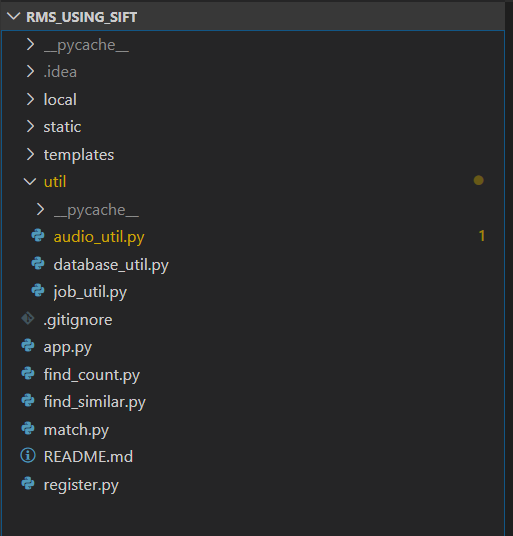
\includegraphics[scale=0.7]{file_structure.PNG}
    \caption{File structure of the codebase}
    \label{fig:file_codebase}
  \end{figure}

\section{File Contents}

\subsection{register.py}
\pythonexternal{codes/register.py}

\subsection{match.py}
\pythonexternal{codes/match.py}

\subsection{audio-util.py}
\pythonexternal{codes/audio_util.py}

\subsection{database-util.py}
\pythonexternal{codes/database_util.py}

\subsection{find-count.py}
\pythonexternal{codes/find_count.py}

\subsection{find-similar.py}
\pythonexternal{codes/find_similar.py}

\subsection{job-util.py}
\pythonexternal{codes/job_util.py}


% \end{appendices}

\end{document}

